\subsection{分段线形插值}


\frame{
$n$次插值是根据给定的$y = f(x)$函数表构造代数多项式$P_n(x)$
\begin{center}
$\Downarrow$
\end{center}
$P_n(x)$为$n$次插值函数,可以近似替代$y = f(x)$。
对于$n$次插值,随着插值节点的增加,插值多项式的次数也会增加。其误差:
\begin{equation*}
E_N (x) = \frac{(x - x_0)(x - x_1) \cdots (x - x_N ) f^{(N+1)}(c)}{(N + 1)!}
\end{equation*}
for some value $c = c(x)$ that lies in the interval $[a, b]$.
\begin{center}
$\Downarrow$
\end{center}
\begin{block}{问题}
插值多项式的次数越高,插值多项式$P_n(x)$与$f(x)$的误差就会越小?
\end{block}
}

\frame{
\frametitle{例}
给定函数
\begin{equation*}
f(x) = \frac{1}{1+25x^2} \ \ \ \ (-1 \le x \le 1)
\end{equation*}
取等间距插值节点$x_i = -1 + \frac{1}{5}i (i = 0, 1, \ldots, 10)$,试建立插值多项式$P_{10}(x)$,并考察$P_{10}(x)$与$f(x)$的误差。
\begin{center}
$\Downarrow$
\end{center}
由Lagrange型$n$次插值公式可得:
\begin{equation*}
P_{10}(x) = \sum_{i=0}^{10} f(x_i) L_i(x)
\end{equation*}
}

\frame{
其中
\begin{equation*}
x_i = -1 + \frac{1}{5}i \ \ \ \ (i = 0, 1, \ldots, n)
\end{equation*}

\begin{equation*}
f(x_i) = \frac{1}{1 + 25x_i^2} \ \ \ \ (i = 0, 1, \ldots, n)
\end{equation*}


\begin{equation*}
L_i(x) = \frac{(x- x_0)\cdots(x- x_{i-1})(x- x_i)\cdots(x- x_10)}{(x_i-x_0)\cdots(x_i-x_{i-1})(x_i-x_{i+1})\cdots(x_i-x_10)} \ \ \ \ (i = 0, 1, \ldots, n)
\end{equation*}
}

\frame{
\frametitle{Runge(龙格)现象}
下图为函数$f(x)= \frac{1}{1+25x^2}$和$y=P_{10}(x)$的图形。
\begin{figure}
\begin{center}
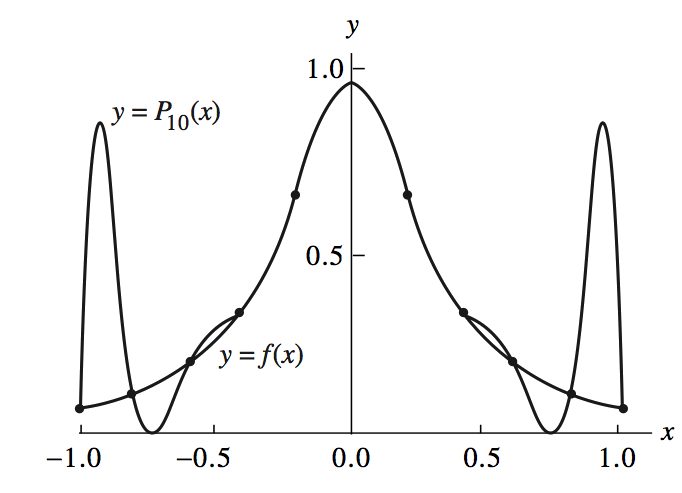
\includegraphics[width=40mm]{chap-3/fig_4-17.png}
\end{center}
\end{figure}
从该图可以观察到:
\begin{itemize}
\item 在原点附近能较好的逼近$f(x)$,
\item 在其他地方$f(x)$和$P_{10}(x)$的误差较大,
\item 越靠近两个端点$-1$和$1$,误差越大,还出现了激烈震荡现象
\end{itemize}
\begin{center}
$\Downarrow$ \\
Runge(龙格)现象
\end{center}
}


\frame{
\begin{center}
Runge(龙格)现象 \\
$\Downarrow$
\end{center}
高次插值多项式并不一定能很好地近似代替被插值函数。

如果给定的插值节点较多,
\begin{center}
$\Downarrow$
\end{center}
\begin{block}{分段插值}
需要把插值区间分为若干段,在每个分段上使用低次插值多项式来近似代替函数$f(x)$
\end{block}
}

\frame{
\frametitle{分段线性插值}
根据给定的函数$f(x)$的函数表
\begin{table}
\begin{tabular}{| c | c | c | c |}
\hline
$x$ & $x_0$ & $\cdots$ & $x_n$ \\
\hline
$y = f(x)$ & $y_0$ & $\cdots$ & $y_n$ \\
\hline
\end{tabular}
\end{table}
构造函数$P(x)$满足条件:
\begin{itemize}
\item $P(x)$在$[x_i, x_{i+1}]$ $(i = 0, 1, \ldots, n-1)$上为不超过一次的代数多项式
\item $P(x_i) = y_i$ ($i = 0, 1, \ldots, n$)
\end{itemize}
\begin{center}
$\Downarrow$
\end{center}
$P(x)$为分段线性插值函数。
}

\frame{
\frametitle{分段线性插值函数}
分段线性插值的目的:分段构造$P(x)$来近似代替$f(x)$。
\begin{equation*}
P(x) = \left\{
\begin{array}{c c}
\frac{x -x_1}{x_0 - x_1} y_0 + \frac{x -x_0}{x_1 - x_0} y_1 & (x_0 \le x \le x_1) \\
\frac{x -x_2}{x_1 - x_2} y_1 + \frac{x -x_1}{x_2 - x_1} y_2 & (x_1 \le x \le x_2) \\
\vdots & \vdots  \\
\frac{x -x_n}{x_{n-1} - x_n} y_{n-1} + \frac{x - x_{n-1}}{x_n - x_{n-1}} y_n & (x_{n-1} \le x \le x_n) \\
\end{array}
\right.
\end{equation*}
}


\frame{
\frametitle{分段线性插值函数也可以由插值基函数组合而成}
设$L_0(x)$, $L_1(x)$, $\cdots$, $\L_n(x)$为线性函数:
\begin{equation*}
L_0(x) = \left\{
\begin{array}{l l}
\frac{x -x_1}{x_0 - x_1}  & (x_0 \le x \le x_1) \\
0 & (x_1 < x \le x_n) \\
\end{array}
\right.
\end{equation*}

\begin{equation*}
L_i(x) = \left\{
\begin{array}{l l}
\frac{x -x_{i-1}}{x_i - x_{i-1}}  & (x_{i-1} \le x \le x_i) \\
\frac{x -x_{i+1}}{x_i - x_{i+1}}  & (x_i < x \le x_{i+1}) \\
0 &  x \in [a, b] - [ x_{i-1},  x_{i+1} ]  \ \ \ ( i = 1, 2, \ldots, n-1 ) \\
\end{array}
\right.
\end{equation*}

\begin{center}
$\vdots$
\end{center}

\begin{equation*}
L_n(x) = \left\{
\begin{array}{l l}
\frac{x -x_{n-1}}{x_n - x_{n-1}}  & (x_{n-1} \le x \le x_n) \\
0 & (x_0 < x < x_{n-1}) \\
\end{array}
\right.
\end{equation*}
}

\frame{
分段线性插值函数的另外一种形式:
\begin{equation*}
P(x) = \sum_{i=0}^n y_i L_i(x)
\end{equation*}

\begin{block}{分段线性插值算法}
\begin{itemize}
\item 读入插值节点$x_i$,$y_i$ ($i=0, 1, \ldots, n$)和点$xx$
\item 对$i=0, 1, \ldots, n$做:
\begin{itemize}
\item 如果$xx<x_i$,则
\item $yy = \frac{xx - x_i}{x_{i-1} -x_i} y_{i-1} + \frac{xx - x_{i-1}}{x_i - x_{i-1}} y_i$
\item 输出点$xx$相对应的函数近似值$yy$
\end{itemize}
\item 结束
\end{itemize}
\end{block}
}

\frame{
\begin{block}{定理}
给定如下表所示$y = f(x)$的函数表,令$a = x_0$,$b = x_n$,$f(x) \in C^1 [a, b]$ ,
$f^{(2)}(x)$在$ [a, b]$上存在,
\begin{table}
\begin{tabular}{| c | c | c | c |}
\hline
$x$ & $x_0$ & $\cdots$ & $x_n$ \\
\hline
$y = f(x)$ & $y_0$ & $\cdots$ & $y_n$ \\
\hline
\end{tabular}
\end{table}
$P(x)$是$f(x)$的分段线性插值函数,则有:
\begin{equation*}
|R(x)| = |f(x) - P(x)| \le \frac{h^2}{8} M
\end{equation*}
其中$h = \max_{0 \le i \le n-1} |x_{i+1} - x_i|$;$M = \max_{a \le x \le b} |f^{(2)}(x)|$。
\end{block}
}



\subsection{Hermite插值}

\frame{
在某些实际问题中,为了保证插值函数更好地逼近被插值函数$f(x)$,
\begin{itemize}
\item 插值函数在插值节点上的值与被插值函数$f(x)$在插值节点上的值相等
\item 插值函数在插值节点上的{\Large 导数值}与被插值函数$f(x)$在插值节点上的{\Large 导数值}相等
\end{itemize}
\begin{center}
$\Downarrow$ \\ \vspace{5mm}
{\huge Hermite插值}
\end{center}
}


\frame{
\frametitle{三次Hermite插值}
给定如下表所示$y = f(x)$的函数表,
\begin{table}
\begin{tabular}{| c | c | c |}
\hline
$ x $ & $x_0$ &  $x_1$ \\
\hline
$y = f(x)$ & $y_0$ & $y_1$ \\
\hline
$y' = f'(x)$ & $m_0$ & $m_1$ \\
\hline
\end{tabular}
\end{table}
构造函数$H(x)$满足条件:
\begin{itemize}
\item $H(x)$为不超过三次的代数多项式
\item $H(x_0) = y_0$,$H(x_1) = y_1$;$H'(x_0) = m_0$,$H'(x_1) = m_1$ 
\end{itemize}
\begin{center}
$\Downarrow$ \\ \vspace{5mm}
$H(x)$为三次Hermite插值函数。
\end{center}
}


\frame{
设
\begin{equation*}
H(x) = y_0 h_0(x) + y_1 h_1(x) + m_0 H_0(x) + y_1 H_1(x) 
\end{equation*}
其中$h_0(x)$,$h_1(x)$,$H_0(x)$和$H_1(x)$为不超过三次的代数多项式,且满足:
\begin{table}
\begin{tabular}{| c | c c | c c|}
\hline
& 函数值 & & 导数值 & \\
& $x_0$ & $x_1$ & $x_0$ & $x_1$ \\
\hline
$h_0(x)$ & $1$ & $0$ & $0$ & $0$ \\
\hline
$h_1(x)$ & $0$ & $1$ & $0$ & $0$ \\
\hline
$H_0(x)$ & $0$ & $0$ & $1$ & $0$ \\
\hline
$H_1(x)$ & $0$ & $0$ & $0$ & $1$ \\
\hline
\end{tabular}
\end{table}
}

\frame{
\frametitle{构造函数$h_0(x)$}
当$x = x_1$时,函数$h_0(x)$的值为$0$,
同时,函数$h_0(x)$的导数也为$0$,
\begin{center}
$\Downarrow$
\end{center}
函数$h_0(x)$必有因子$(x-x_1)^2$。
\begin{center}
$\Downarrow$
\end{center}
另外,$h_0(x)$是一个不超过三次的代数多项式,
\begin{center}
$\Downarrow$
\end{center}
\begin{equation*}
h_0(x) = [a + b(x-x_0)] \left( \frac{x - x_1}{x_0 - x_1} \right)^2
\end{equation*}
其中$a$和$b$为待定系数。
}

\frame{
\frametitle{求解$h_0(x)$}
由$h_0(x_0) = 1$可得$a=1$。

\begin{equation*}
h'_0(x) = b \left( \frac{x - x_1}{x_0 - x_1} \right)^2 + [1 + b (x-x_0)] \times 2 \times \left( \frac{x - x_1}{x_0 - x_1} \right)^ \times \frac{1}{x_0 - x_1}
\end{equation*}
$h'_0(x_0) = 0$
\begin{center}
$\Downarrow$
\end{center}
\begin{equation*}
b = \frac{2}{x_1 - x_0}
\end{equation*}

\begin{center}
$\Downarrow$
\end{center}

\begin{equation*}
h_0 (x) = \left ( 1 + 2 \frac{x- x_0}{x_1 - x_0} \right) \left ( \frac{x-x_1}{x_0 - x_1} \right)^2
\end{equation*}

同理可得
\begin{equation*}
h_1 (x) = \left ( 1 + 2 \frac{x- x_1}{x_0 - x_1} \right) \left ( \frac{x-x_0}{x_1 - x_0} \right)^2
\end{equation*}
}

\frame{
\frametitle{构造函数$H_0(x)$}
由于$H_0(x)$在$x_0$处的函数值为$0$,在$x_1$处不仅函数值为$0$,而且微商也为$0$
\begin{center}
$\Downarrow$
\end{center}
$H_0(x)$必有因子$(x - x_0)(x - x_1)^2$
\begin{center}
$\Downarrow$
\end{center}
又因为$H_0(x)$是一个不超过三次的代数多项式,而$(x - x_0)(x - x_1)^2$已经是一个三次多项式,从而$H_0(x)$可表示为:
\begin{equation*}
H_0(x) = c (x - x_0) \left( \frac{x - x_1}{x_0-x_1} \right)^2
\end{equation*}
其中$c$为待定系数。
}

\frame{
\frametitle{求解$H_0(x_0) $}
对$H_0(x_0)$求微商,可得:
\begin{equation*}
H'_0(x) = c \left[ \left( \frac{x - x_1}{x_0-x_1} \right)^2 + 2 (x - x_0) \frac{X-X_1}{(x_0 - x_1)^2} \right]
\end{equation*}
\begin{center}
$\Downarrow$
\end{center}
由$H'_0(x) = 1$,可得$c=1$,于是:
\begin{equation*}
H_0(x) =  (x - x_0) \left( \frac{x - x_1}{x_0-x_1} \right)^2
\end{equation*}
\begin{center}
$\Downarrow$
\end{center}
同理可得:
\begin{equation*}
H_1(x) =  (x - x_1) \left( \frac{x - x_0}{x_1-x_0} \right)^2
\end{equation*}
}

\frame{
综上所述,我们可得到三次Hermite插值公式
\begin{equation*}
\begin{array}{l c l}
H(x) & = & y_0 h_0(x) + y_1 h_1(x) + m_0 H_0(x) + m_1 H_1(x) \\
& = & \left ( 1 + 2 \frac{x- x_0}{x_1 - x_0} \right) \left ( \frac{x-x_1}{x_0 - x_1} \right)^2 y_0 + \left ( 1 + 2 \frac{x- x_1}{x_0 - x_1} \right) \left ( \frac{x-x_0}{x_1 - x_0} \right)^2 y_1\\
&  & +  (x - x_0) \left( \frac{x - x_1}{x_0-x_1} \right)^2 m_0 + (x - x_1) \left( \frac{x - x_0}{x_1-x_0} \right)^2 m_1 \\
\end{array}
\end{equation*}
}

\frame{
\begin{block}{定理}
设$H(x)$是$f(x)$的三次Hermite插值函数,$[a, b]$是包含$x_0$,$x_1$的任一区间,
并设$f(x) \in C^3 [a, b]$,$f^{(4)}(x)$在 $[a, b]$上存在,则对任意给定的$x \in [a, b]$,总存在一点$\xi \in [a, b]$,使得
\begin{equation*}
R(x) = f(x) - H(x) = \frac{f^{(4)}(\xi)}{4!} (x - x_0)^2 (x -x_1)^2
\end{equation*}
其中$\xi$依赖于$x$。
\end{block}
}





\frame{
\frametitle{$2n+1$次Hermite插值}
给定$y = f(x)$的函数表,
\begin{table}
\begin{tabular}{| c | c | c | c | c |}
\hline
$x$ & $x_0$ & $x_1$ & $\cdots$ & $x_n$ \\
\hline
$y = f(x)$ & $y_0$ & $y_1$ & $\cdots$ & $y_n$ \\
\hline
$y' = f'(x)$ & $m_0$ & $m_1$ & $\cdots$ & $m_n$ \\
\hline
\end{tabular}
\end{table}
构造函数$H(x)$满足条件:
\begin{itemize}
\item $H(x)$为不超过$2n+1$次的代数多项式
\item $H(x_i) = y_i$,$H'(x_i) = m_i$ ($i = 0, 1, \ldots, n$)
\end{itemize}
则称$H(x)$为$2n+1$次Hermite插值函数。
}

\frame{
设
\begin{equation*}
H(x) = \sum_{i=0}^n \left[ y_i h_i (x) + m_i H_i(x) \right]
\end{equation*}
$i = 0, 1, \ldots, n$,其中$h_i(x)$和$H_i(x)$为不超过$2n+1$的代数多项式,且满足
\begin{table}
\begin{tabular}{| c | c c c c| c c c c|}
\hline
& & 函数值 & & & & 导数值 & & \\
& $x_0$ & $x_1$ & $\cdots$ & $x_n$ & $x_0$ & $x_1$ & $\cdots$ & $x_n$ \\
\hline
$h_0(x)$ & $1$ & $0$ & $\cdots$ & $0$  & $0$ & $0$ & $\cdots$ & $0$ \\
\hline
$h_1(x)$ & $0$ & $1$ & $\cdots$ & $0$  & $0$ & $0$ & $\cdots$ & $0$ \\
\hline
$\vdots$ & $\vdots$ & $\vdots$ & $\vdots$ & $\vdots$  & $\vdots$ & $\vdots$ & $\vdots$ & $\vdots$ \\
\hline
$h_n(x)$ & $0$ & $0$ & $\cdots$ & $1$  & $0$ & $0$ & $\cdots$ & $0$ \\
\hline
$H_0(x)$ & $0$ & $0$ & $\cdots$ & $0$  & $1$ & $0$ & $\cdots$ & $0$ \\
\hline
$H_1(x)$ & $0$ & $0$ & $\cdots$ & $0$  & $0$ & $1$ & $\cdots$ & $0$ \\
\hline
$\vdots$ & $\vdots$ & $\vdots$ & $\vdots$ & $\vdots$  & $\vdots$ & $\vdots$ & $\vdots$ & $\vdots$ \\
\hline
$H_n(x)$ & $0$ & $0$ & $\cdots$ & $0$  & $0$ & $0$ & $\cdots$ & $1$ \\
\hline
\end{tabular}
\end{table}
}


\frame{
\frametitle{构造$h_0(x)$}
$h_0(x) = h'_0(x) = 0$
\begin{center}
$\Downarrow$
\end{center}
$h_0(x)$必有因子$[(x-x_1)(x-x_2)\cdots(x-x_n)]^2$。
\begin{center}
$\Downarrow$
\end{center}
$h_0(x)$为不超过$2n+1$次的代数多项式,
\begin{center}
$\Downarrow$
\end{center}
\begin{equation*}
h_0(x) = (ax + b) L_0^2(x)
\end{equation*}
其中$a$和$b$为待定常数;
\begin{equation*}
L_0(x) = \frac{(x-x_1)(x-x_2)\cdots(x-x_n)}{(x_0-x_1)(x_0-x_2)\cdots(x_0-x_n)}
\end{equation*}
}

\frame{
因为$h_0(x_0) =1$,故有$a x_0 + b = 1$,即$b = 1 -a x_0$。
\begin{center}
$\Downarrow$
\end{center}
对$h_0(x)$求一介导数,可得:
\begin{equation*}
h'_0(x) = a L_0^2(x) + 2 (ax+b) L_0(x) L'_0(x)
\end{equation*}
由$h'_0(x_0) = 0$,故有:
\begin{equation*}
h'_0(x_0) = a + 2 L'_0(x) = 0
\end{equation*}
\begin{center}
$\Downarrow$
\end{center}
\begin{equation*}
a = -2 L'_0 (x_0)
\end{equation*}
\begin{equation*}
b = 1 + 2 x_0 L'_0 (x_0)
\end{equation*}
\begin{equation*}
h_0(x) = [1 - 2 (x - x_0) L'_0 (x_0)] L^2_0(x)
\end{equation*}
}

\frame{
为求$L'_0(x)$,对$L_0(x)$两边取对数可得
\begin{equation*}
\begin{array}{l l}
\ln [L_0(x)] = & \ln(x -x_1) + \ln(x -x_2) + \cdots + \ln(x -x_n) \\
& - \left[ \ln(x_0 -x_1) + \ln(x_0 -x_2) + \dots + \ln(x_0 -x_n) \right] \\
\end{array}
\end{equation*}
对上式两边求导数可得:
\begin{equation*}
\frac{1}{L_0(x)} L'_0(x) = \sum_{j=1}^n \frac{1}{x - x_j}
\end{equation*}
\begin{center}
$\Downarrow$
\end{center}
\begin{equation*}
 L'_0(x) = L_0(x) \left( \sum_{j=1}^n \frac{1}{x - x_j} \right)
\end{equation*}
由此可得
\begin{equation*}
 L'_0(x_0) = \sum_{j=1}^n \frac{1}{x_0 - x_j} 
\end{equation*}
}

\frame{
可以得到:
\begin{equation*}
h_0(x) = \left[ 1 - 2 (x -x_0) \left( \sum_{j=1}^n \frac{1}{x_0 - x_j}  \right) \right]  L_0^2(x)
\end{equation*}

\vspace{5mm}
用同样的方法可以得到:
\begin{equation*}
h_i(x) = \left[ 1 - 2 (x -x_i) \left( \sum_{j=1, j\neq i}^n \frac{1}{x_i - x_j}  \right) \right]  L_i^2(x)
\end{equation*}
其中$i = 0, 1, \ldots, n$
}


\frame{
\frametitle{构造$H_0(x)$}
$H_0(x_0) = 0$和$H_0(x_i) = H'_0(x_i)  =0$,其中$i = 0, 1, \ldots, n$
\begin{center}
$\Downarrow$
\end{center}
$H_0(x)$必有因子$(x - x_0) [(x-x_1)(x-x_2)\cdots(x-x_n)]^2$。
\begin{center}
$\Downarrow$
\end{center}
$H_0(x)$为不超过$2n+1$次的代数多项式,
\begin{center}
$\Downarrow$
\end{center}
\begin{equation*}
H_0(x) = a (x - x_0) L_0^2(x)
\end{equation*}
其中$a$为待定常数;
}

\frame{
对$H_0(x)$求一介导数,可得:
\begin{equation*}
H'_0(x) = a \left[ L_0^2(x) + 2 (x-x_0) L_0(x) L'_0(x) \right] 
\end{equation*}
由$H'_0(x) = 1$可得$a=1$。
于是可以得到:
\begin{equation*}
H_0(x) =  (x - x_0) L_0^2(x)
\end{equation*}

用同样的方法可以得到:
\begin{equation*}
H_i(x) =  (x - x_i) L_i^2(x)
\end{equation*}
其中$i = 0, 1, \ldots, n$
}

\frame{
$2n+1$次Hermite插值为
\begin{equation*}
\begin{array}{r l}
H(x) = &  \sum_{i=0}^n \left[ y_i h_i (x) + m_i H_i(x) \right] \\
 = & \sum_{i=0}^n \left\{ y_i \left[ 1 - 2 (x -x_i) \left( \sum_{j=1, j\neq i}^n \frac{1}{x_i - x_j}  \right) \right]  L_i^2(x) + m_i (x - x_i) L_i^2(x) \right\} \\
\end{array}
\end{equation*}
\begin{block}{定理}
设$H(x)$是$f(x)$的$2n+1$次Hermite插值函数,$[a, b]$是包含$x_0$,$x_1$,$\cdots$,$x_n$的任一区间,
并设$f(x) \in C^{2n+1} [a, b]$,$f^{(2n+2)}(x)$在 $[a, b]$上存在,则对任意给定的$x \in [a, b]$,总存在一点$\xi \in [a, b]$,使得
\begin{equation*}
R(x) = f(x) - H(x) = \frac{f^{(2n+2)}(\xi)}{(2n+2)!} \omega^2(x)
\end{equation*}
其中$\xi$依赖于$x$,$\omega(x) = (x-x_0)(x-x_1)\cdots(x-x_n)$。
\end{block}
}



\subsection{分段三次Hermite插值}

\frame{
给定函数$y = f(x)$ 的函数表
\begin{table}
\begin{tabular}{| c | c | c | c |}
\hline
$x$ & $x_0$ & $\cdots$ & $x_n$ \\
\hline
$y = f(x)$ & $y_0$ & $\cdots$ & $y_n$ \\
\hline
\end{tabular}
\end{table}
构造函数$q(x)$满足条件:
\begin{itemize}
\item $q(x)$在$[x_i, x_{i+1}]$($i = 0, 1, \ldots, n-1$)上为三次代数多项式
\item $q(x_i) = y_i$,$q'(x_i) = m_i$($i = 0, 1, \ldots, n$)
\item $q(x) \in C^1[a, b]$,其中$a = f(x_0)$,$b = f(x_n)$
\end{itemize}
则$q(x)$称为分段三次Hermite插值函数。
其在区间$[x_i, x_{i+1}]$上有
\begin{equation*}
\begin{array}{l c l}
q(x) & = &  \left ( 1 + 2 \frac{x- x_i}{x_{i+1} - x_i} \right) \left ( \frac{x-x_{i+1}}{x_i - x_{i+1}} \right)^2 y_i + \left ( 1 + 2 \frac{x- x_{i+1}}{x_i - x_{i+1}} \right) \left ( \frac{x-x_i}{x_{i+1} - x_i} \right)^2 y_{i+1} \\
&  & +  (x - x_i) \left( \frac{x - x_{i+1}}{x_i-x_{i+1}} \right)^2 m_i + (x - x_{i+1}) \left( \frac{x - x_i}{x_{i+1}-x_i} \right)^2 m_{i+1} \\
\end{array}
\end{equation*}
}

\frame{
分段三次Hermite插值函数$q(x)$可由插值基函数组合而成:
若在插值区间$[a,b]$上定义一组分段三次Hermite插值基函数$h_i(x)$和$H_i(x)$($i = 0, 1, \ldots, n$),则可得
\begin{equation*}
q(x) = \sum_{i=0}^n [y_i h_i(x) + m_i H_i(x)]
\end{equation*}
其中$h_i(x)$和$H_i(x)$分别为
\begin{equation*}
h_0(x) = \left\{
\begin{array}{c c}
\left( 1 + 2 \frac{x-x_0}{x_1-x_0} \right) \left( \frac{x-x_1}{x_0-x_1}  \right)^2 & (x_0 \le x \le x_1) \\
 0 & (x_1 < x \le x_n)\\
\end{array}
\right.
\end{equation*}

\begin{equation*}
h_i(x) = \left\{
\begin{array}{c c}
\left( 1 + 2 \frac{x-x_i}{x_{i-1}-x_i} \right) \left( \frac{x-x_{i-1}}{x_i-x_{i-1}}  \right)^2 & (x_{i-1} \le x \le x_i) \\
\left( 1 + 2 \frac{x-x_i}{x_{i+1}-x_i} \right) \left( \frac{x-x_{i+1}}{x_i-x_{i+1}}  \right)^2 & (x_i < x \le x_{i+1}) \\
 0 & [a, b] - [x_{i-1},  x_{i+1}]\\
\end{array}
\right.
\end{equation*}

\begin{equation*}
h_n(x) = \left\{
\begin{array}{c c}
\left( 1 + 2 \frac{x-x_n}{x_{n-1}-x_n} \right) \left( \frac{x-x_{n-1}}{x_n-x_{n-1}}  \right)^2 & (x_{n-1} \le x \le x_n) \\
 0 & (x_0 \le x < x_{n-1})\\
\end{array}
\right.
\end{equation*}
}

\frame{
\begin{equation*}
H_0(x) = \left\{
\begin{array}{c c}
(x -x_0) \left( \frac{x-x_1}{x_0-x_1} \right)^2  & (x_0 \le x \le x_1) \\
 0 & (x_1 < x \le x_n)\\
\end{array}
\right.
\end{equation*}

\begin{equation*}
H_i(x) = \left\{
\begin{array}{c c}
(x -x_i) \left( \frac{x-x_{i-1}}{x_i-x_{i-1}} \right)^2  & (x_{i-1} \le x \le x_i) \\
(x -x_i) \left( \frac{x-x_{i+1}}{x_i-x_{i+1}} \right)^2  & (x_i < x \le x_{i+1}) \\
 0 & [a, b] - [x_{i-1},  x_{i+1}]\\
\end{array}
\right.
\end{equation*}

\begin{equation*}
H_n(x) = \left\{
\begin{array}{c c}
(x -x_n) \left( \frac{x-x_{n-1}}{x_n-x_{n-1}} \right)^2  & (x_{n-1} \le x \le x_n) \\
 0 & (x_0 \le x < x_{n-1})\\
\end{array}
\right.
\end{equation*}
}


\frame{
\begin{block}{定理}
设如下表所示的函数表,令$a=x_0$,$b=x_n$,$f(x) \in C^{(3)} [a, b]$,$f^{(4)}(x)$在 $[a, b]$上存在,$q(x)$是$f(x)$的分段三次Hermite插值函数,则有
\begin{equation*}
| R(x) | = | f(x) - q(x) | \le \frac{h^4}{384} M
\end{equation*}
其中
\begin{equation*}
h= \max_{0 \le i \le n-1} |x_{i+1} - x_i|
\end{equation*}
\begin{equation*}
M = \max_{0 \le i \le n-1} |f^{(4)}(x)|
\end{equation*}
\end{block}
\begin{table}
\begin{tabular}{| c | c | c | c | c |}
\hline
$x$ & $x_0$ & $x_1$ & $\cdots$ & $x_n$ \\
\hline
$y = f(x)$ & $y_0$ & $y_1$ & $\cdots$ & $y_n$ \\
\hline
$y' = f'(x)$ & $m_0$ & $m_1$ & $\cdots$ & $m_n$ \\
\hline
\end{tabular}
\end{table}
}

